\documentclass[conference]{IEEEtran}
\IEEEoverridecommandlockouts
% The preceding line is only needed to identify funding in the first footnote. If that is unneeded, please comment it out.
\usepackage{cite}
\usepackage{amsmath,amssymb,amsfonts}
\usepackage{algorithmic}
\usepackage{graphicx}
\usepackage{textcomp}
\usepackage{xcolor}
\usepackage[colorlinks=true,linkcolor=blue,urlcolor=cyan]{hyperref}

\def\BibTeX{{\rm B\kern-.05em{\sc i\kern-.025em b}\kern-.08em
    T\kern-.1667em\lower.7ex\hbox{E}\kern-.125emX}}
\begin{document}

\title{A Hybrid Approach to Scientific Software Package Management on a HPC Cluster}

\author{\IEEEauthorblockN{Qiyang Hu}
\IEEEauthorblockA{\textit{Institute for Digital Research and Education} \\
\textit{University Of California, Los Angeles}\\
Los Angeles, California, USA \\
huqy@idre.ucla.edu}
\and
\IEEEauthorblockN{Shao-Ching Huang}
\IEEEauthorblockA{\textit{Institute for Digital Research and Education} \\
\textit{University Of California, Los Angeles}\\
Los Angeles, California, USA \\
schuang@idre.ucla.edu}
}

\maketitle

\begin{abstract}
We present a practical approach for managing the scientific packages in the HPC cluster environment of a research university environment that has a diverse user base.
%%%Having to install and maintain a large number of software packages to support the boradband spectrum of university research motivates the use of a software installation framework to lessen the burden on the HPC operational team. Challenges arise when the framework has to be integrated with in-house package installation pratice already existed. In practice, the in-house installation component is required because not all packages can be satisfactorily covered by a software management framework.
The primary goal is to minimize the HPC operational team's burden of installing and maintaining a large number of software packages to support the broadband spectrum of the university's computational research.
We propose a hybridizing management method that can harness the power of modern software management frameworks and the flexibility of in-house, or ``manual'', installation sources, and at the same time present a coherent view to the end users. The Spack~\cite{gamblin:15} framework was used in this work. Our hybrid approach is applicable to using other framework tools. The manipulation of Spack-generated environment module files and the typical workflow are illustrated and discussed based on our use case.
\end{abstract}

\begin{IEEEkeywords}
software management, environment modules, Spack, HPC 
\end{IEEEkeywords}

\section{Introduction}\label{sec_intro}

%%{\color{gray}(1) General challenge}
%%%Keeping scientific software packages on the HPC cluster up-to-date and easy to use, from a user's view, in a research university environment that has a diverse user base can be a challenge when the number of packages is large.
%%%Keeping scientific computing software packages up-to-date and easy to use for users is of ultimate importance to a successful campus high performance computing (HPC) cluster operation in a research university environment.
%%%In practice, this can pose a challenge on a small operational team when the number of scientific packages on the HPC cluster is large (e.g. in the hundreds that we considered in this work). 
%%%Keeping every software installation up to date and providing persistent support to the diverse user needs are tedious and time-consuming if done manually.
%%%The combinatorial naming and versioning complexities result in large number of package sets (e.g. built by different tool sets and optimized libraries), module files and the corresponding documents that need to be maintained by the operational team. 
%%{\color{gray}(2) framework solution's advantages}
%%%A common solution to this challenge is to use a software management framework, such as EasyBuild\cite{geimer:14} or Spack\cite{gamblin:15}, to simplify or automate the process. 
%%%In a software management framework, the configre-build-deploy process is done in a systematic fashion; such an approach promises to largely improve HPC cluster's operational efficiency. 
%%{\color{gray}(3) framework solution's limitations}
%%%However, as the software management frameworks are still under rapid development, albeit very powerful, a few limitations are noted in practice when other installation sources also exist. One common example is the manually-installed packages not covered in the software management framework.
%%%First, from the cluster operation's standpoint, the restrictions from the frameworks may not be compatible with the site's existing/legacy package installation structure (referred to as manually-installed packages, including those done by in-house installation scripts), even for the most flexible framework solution that we consider in this work (i.e. Spack). ({\color{red} Shall we called it "locally-installed" vs. "framework-installed" instead? "manual" seems misleading.}) 
%%%It is not possible to conveniently plug framework-installed packages into the existing manually-installed structures without significantly altering how the framework works, which is non-trivial.
%%%Second, it is difficult produce a consistent view of available software modules to users when the framework's module file naming conventions are different from that defined by the operation team. 
%%%Third, It is always difficult to manage software and dependencies built outside of the tools. 
%%%Fourth, the framework's systematic handling on library dependencies results in many duplicate builds of the same software; this can create confusion if presented to users at once.
%%%Fifth, we note that a number of new, but less mature, functionalities in the framework are unable to handle corner cases that we encountered in practice. Given the above considerations, it would be ideal to have a way to take advantage of the powerful capability of framework approach and at the same time maintain compatibility complying to the operational team's design goals in terms of scientific package management.

%== Having to install and maintain a large number of software packages to support the broadband spectrum of university research motivates the use of a software installation framework, such as EasyBuild\cite{geimer:14} or Spack\cite{gamblin:15}, to automate the processes and thus lessen the burden on HPC operational teams. 
%== However, challenges arise when the framework has to be integrated with in-house package installation practices already existed. In practice, the in-house installation component is required because not all packages can be satisfactorily managed within a software management framework.

A recent challenge for HPC system administrators to adopt the software installation frameworks (e.g. EasyBuild\cite{geimer:14} or Spack\cite{gamblin:15}) is that those frameworks may have to be integrated with in-house package installation practices already existed. In practice, the in-house installation component is required because not all packages can be satisfactorily managed within a software management framework.

%%{\color{gray}(4) our approach and values/contributions of our work}
In this work, we propose a practical approach for HPC cluster operational teams to manage software packages by hybridizing the framework and manual-based installation methods. 
%==From a software design point of view, 
Conceptually, our central idea is to add a layer above the existing software management frameworks, where a workflow is introduced to manage applications built either by the framework or by manual installation to enable flexible customization, complying to the existing structure of the HPC cluster environment.
The framework-installed and manually-installed packages are kept separate by design, so it will allow future changes of the HPC environment, including the possibility of adopting another installation framework.
In this paper, we adopt Spack as the package management framework. The proposed approach is applicable to using other software management frameworks. We consider the deployment of the hybrid approach on UCLA Hoffman2 Cluster where an in-house package installation structure already exists.
A main contribution of this work is a noble way to manipulate and re-organize the environment modules and offer a practical, automated and script-able workflow to build and maintain the packages, and to provide a coherent view to end users.


%%%\section{Managing Module Files} \label{sec_modulefiles}

%%%\subsection{Module file management in Spack}
%\section{Defining modulefile structures in user level} \label{subsec_redefine_h2_modulefiles}
\section{Modulefile structure cutomization} \label{subsec_redefine_h2_modulefiles}

%%{\color{gray}General}
%%%Adding a flexible management layer on top of framework rely on the exploration of the detailed module file structure generated by the framework.
%%%In Spack, module files are automatically generated during the installation and it systematically collects all dependent libraries and provide the corresponding modules. 
%%%The structure and format for module files are controlled by Spack's yaml scripts (\verb|config.yaml| and \verb|modules.yaml|).
%%% and it can generate both flat and hierarchical structured module files at the same time. 

%%{\color{gray}Flat}
%%%The flat TCL/C module file structure generated by Spack has a straight-forward naming scheme under the root place with simple listing of package names 
%%%concatenating the version and compiler/mpi information with unique hash code. 
%%%As shown in Fig. \ref{fig:spack_flat} of an example that we installed on Hoffman2, different installations of each package are stored in the corresponding directory as TCL/C module files with a name concatenating the application version, compiler name, compiler version, and the mpi name and version. Plus, the TCL/C module files appends the unique hash code in order to distinguish the duplication names from minor difference of installations with the same version and same compiler/mpi info.
%%%
%%%\begin{figure}[htbp]
%%%  \centerline{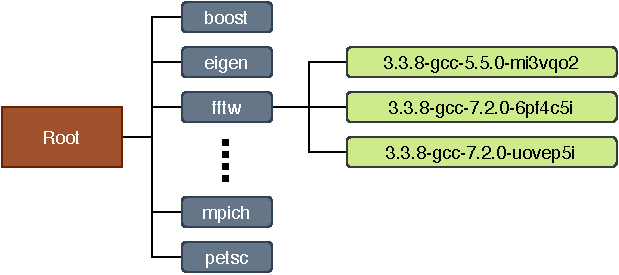
\includegraphics[width=\linewidth]{figures/spack_flat}}
%%%  \caption{Flat structure of module files generated by Spack}
%%%  \label{fig:spack_flat}
%%%\end{figure}

%%{\color{gray}Hierarchical}
%%%At the same time, the hierarchical module files generated by Spack follows the typical Core/Compiler/MPI structures
%%%Fig.~\ref{fig:spack_hier} shows an example of our modules.yaml configuration on Hoffman2. 
%%%It can be noticed that the software installations are organized 
%%%in a convoluted way.
%%%, which means the applications under ``Core'' are the simplest with only dependency on system libraries, the ones under ``Compiler''s are dependent on the Spack-installed compilers only, the ones under ``MPI'' are dependent on both compilers and mpis. In Fig.~\ref{fig:spack_hier} we introduced customized ``openblas'' category to test the customization capabilities of Spack's modules.yaml. It can be understood as the in-between level of Compiler and MPI, which obviously adds more complexity in the MPI level directory. Every package installed is listed as a folder as its name under the corresponding directory levels. The module files for different versions are \texttt{lua} files with \texttt{.lua} extension and have a simpler name with its own version plus the unique hash code if necessary.

%%%\begin{figure}[htbp]
%%%  \centerline{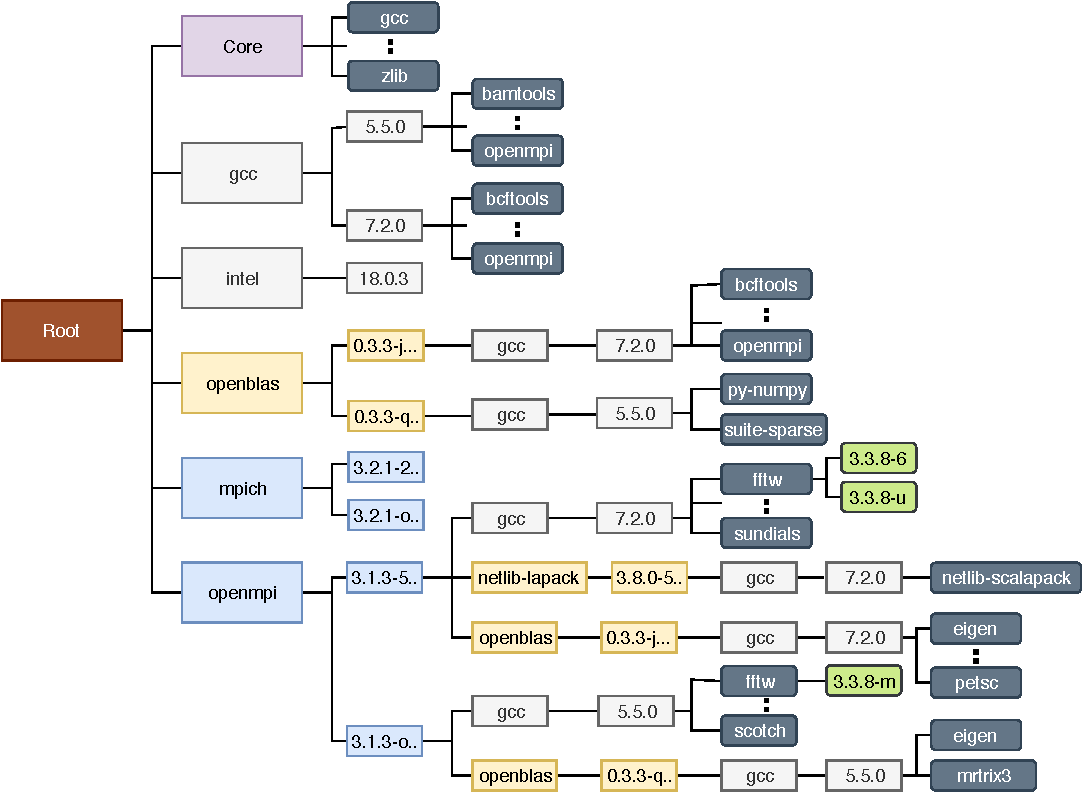
\includegraphics[width=\linewidth]{figures/spack_hier}}
%%%  \caption{Hierarchical structure of module files generated by Spack}
%%%  \label{fig:spack_hier}
%%%\end{figure}


Adding a flexible management layer on top of framework requires traversing the module file structure generated by the software management framework.
From our experiences in practice, configuration through Spack's YAML files is not flexible enough for our needs.
%%%Due to the systematic installation, the minor tweaks of flags and options for the same packages will be considered as different versions. 
%%%But the naming scheme from Spack yaml script is impossible to cover all the cases. 
Specifically, Spack's installation processes create multiple duplications of installed packages and libraries. Presenting all versions of the Spack-built software packages, with embeded unique hash codes in the package's display names at once, introduces big confusion to the end users.
In addition, the predefined hierarchical structure create by Spack is quite rigid and incompatible for our pre-existed cluster environment. There seems to be no easy way to customize it. 
%%%In our Hoffman2 system, about 1/3 of existing packages in the HPC cluster has to be managed with the traditional manual way. 
%%%We need to design a neat hierarchical module file structure so that the module files from Spack can have a unique mapping and the manually generated module files can also comply the definition.

Based on our experience, also motivated by the operation of other large-scale HPC clusters (e.g. TACC Stampede), we first propose the module files to be organized in a simple structure as shown in Fig. \ref{fig:h2_new_hier}, where the MPI level is nested in the compiler level. 
The versions of compilers and MPIs follow the convention in Spack. 
%%%We will use \texttt{lua} format which means the module files will have \texttt{.lua} extension. 
%%%\texttt{modulefiles} sub-directory is preserved for denoting to store the installed packages' module files from the upper directories from the corresponding compilers, or MPIs or both. 
Additional categories can be nested in Compiler level or Compiler+MPI levels if needed. Such a hierarchical organization, in contrast to a flat one, can prevent the users from loading incompatible software packages (e.g. libraries compiled with different MPI implementations) in practice.

\begin{figure}[htbp]
  \centerline{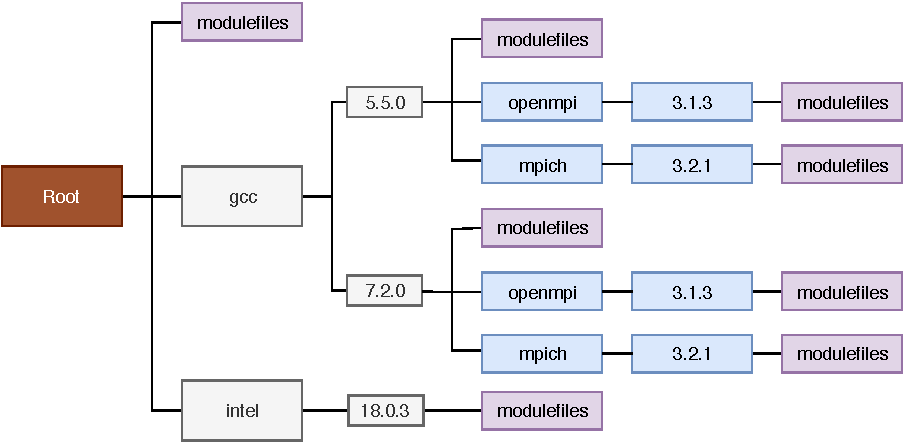
\includegraphics[width=\linewidth]{figures/h2_new_hier}}
  \caption{Newly defined hierarchical structure of module files in Hoffman2}
  \label{fig:h2_new_hier}
\end{figure}

\section{Hybridization of modulefiles}\label{subsec_modulefile_processing}

With our own design of module file structure defined in Section \ref{subsec_redefine_h2_modulefiles}, hybridization of the framework-based (Spack) and the manually-installed systems is achieved by implementing a configurable procedure to (1) traverse the modulefile tree generated by Spack, (2) filter out the undesirable packages (e.g. duplicates and not-to-be-supported packages), and (3) export the results to a new modulefile tree which will be the default module path for end users.

We use JSON to express the information of the packages that our HPC operational team will support, i.e. visible to end users. An example of a JSON file is listed below:
%%%, where only 3 packages will be supported and the versions are listed by concatenating the compiler's information:

{\small
\begin{verbatim}
{   "bowtie2": {
        "name_in_spack": "bowtie2",
        "version": [
            "2.3.4.1-gcc-7.2.0",
            "2.3.4.1-gcc-5.5.0"
        ],
        "default": "2.3.4.1"
    },
}
\end{verbatim}
}

%%%where the main name in the json object pair is the application name preferred by system admins. The \verb|name_in_spack| is the name used in Spack. It can be blank if there is no cooresponding one in Spack. The \verb|version| keeps the application version information and the corresponding compilers. The default version that will be shown or selected by the \verb|Lmod| system.

Our approach takes advantage of Spack's capability of generating both flat and hierarchical module files by enabling them in modules.yaml configuration file. As shown in Fig. \ref{fig:modulefilter_flowchart}, we first traverse over Spack's hierarchical module structures to obtain the hierarchical information about the installed packages and the hash codes generated from Spack. All collected information is stored in a SQLite database. Then we traverse Spack's flat-structured module files to find the ones in the database with the same hash code. By cross-checking the customized JSON file to decide the display option for the packages we can create the final modulefile tree in the destination directory. This process specifically include the following steps:

\begin{itemize}
    \item Using \texttt{tcl2lua.tcl} script to convert the \texttt{TCL/C} module file to \texttt{lua} format.
    \item Pre-pending \texttt{MODULEPATH} to enable the dynamically showing of available module files under the corresponding Compiler/MPI directories if necessary.
    \item Adding \texttt{family} to guarantee users can only load one compiler or MPI stack at a time, if necessary.
    \item Specifying the default version for the packages by generating \texttt{.version} file in the destination package modulefile folder.
\end{itemize}

\begin{figure}[htbp]
  \centerline{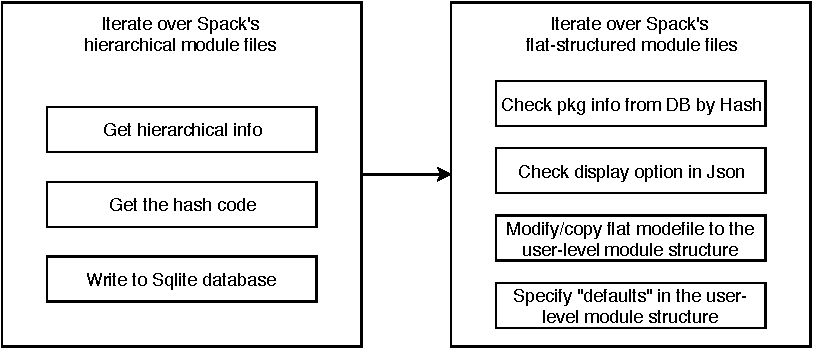
\includegraphics[width=\linewidth]{figures/modulefilter_flowchart}}
  \caption{Flowchart for the python script to generate the newly defined module file structures for user-level presentations}
  \label{fig:modulefilter_flowchart}
\end{figure}

In the SQLite database, (\verb|apps.db|), there is currently only one table, (\verb|apps|). The schema of the table can be reviewed by \verb|.schema apps| inside the SQLite shell. The detailed scripts is publicly available in a gitlab repository\cite{gitlabrepo}.


\section{Operational workflows} \label{sec_workflow}

The workflow to hybridize the Spack-installed and manually-installed packages as described in Section \ref{subsec_modulefile_processing} is illustrated in Figure \ref{fig:spack_h2_hybrid_flow}, showing an example of the process of installing a package on the HPC cluster for a system admin, starting from recieving an installation request, logging into a dedicated account (\verb|$SPACK_ADMIN|) and ending with displaying the module(s) to end users. It should be noted that the workflow can be also taken in any subgroup package environment defined in Spack \cite{spack:20}.

\begin{figure}[htbp]
  \centerline{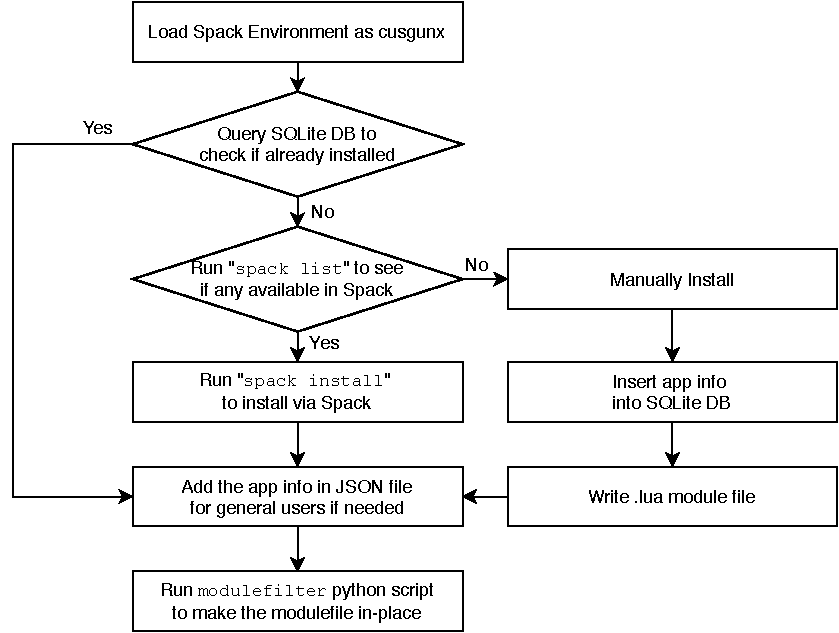
\includegraphics[width=\linewidth]{figures/spack_h2_hybrid_flow}}
  \caption{Workflow to hybridize the Spack-installed and manually-installed packages}
  \label{fig:spack_h2_hybrid_flow}
\end{figure}

%%%A couple of notes are listed below for further explantation:
%%%
%%%\begin{itemize}
%%%    \item All the installation processes are assumed to be taken as a specific non-root user.
%%%    \item The standard SQL \verb|select| query would be used to check if the newly requested package with the specific requested version has been installed on Hoffman2 or not.
%%%    \item If installation is needed, the command \verb|spack list $APPNAME|\cite{spack:20} can be used to check if there is any available package whose name contains \verb|$APPNAME| Spack can install. 
%%%    \item If Spack provides the available package to install, the command \verb|spack install $APPNAME|\cite{spack:20} can be used to install it. As a reference, we installed 180+ packages on Hoffman2 using \verb|spack install| commands. 
%%%    \item For packages needed the manual installation, a SQL \verb|insert| command will be needed to populate the information into the database. It should be noted that the field \verb|apphash| has to leave blank as the flag to denote the installation is not from Spack.
%%%    \item The \verb|lmod| modulefile from manually installed package will needed to be written manually as well. It can be the \verb|TCL/C|-based script or \verb|lua|-based one, since the modulefilter script will do the conversion. The directory for drafting the module file can be arbitrary but has to be consistent with the value of the \verb|flatpath| in the database record inserted above.
%%%    \item The JSON file has to be updated according the schema described in Section \ref{subsec_modulefile_processing}. 
%%%\end{itemize}


\section{Summary} \label{sec_summary}

%== In this work we proposed an approach to hybridize the software management framework and the traditional manual package management. 
%== %The design adds a layer on top of the standard package management framework, in order to take advantage of the powerful framework, the flexibility of the traditional manual management and the desired HPC user interface, via the use of modulefiles constructed to prevent loading incomptabible packages. 
%== The design adds a layer on top of the standard package management framework expecting to take advantage of the powerfule framework while maintaining the management flexibility for manual installations and the customizable HPC user interface. 
%== %With the definition of a customizable module file structure in the HPC cluster environment, the workflow is able to process, filter and integrate the module files from two independent sources (i.e. framework-based and manual-based) to any target modulefile presentation. 
We propose an approach to hybridize the software management framework and the traditional manual package management.
We demonstrate that the workflow is able to to filter and integrate the module files from two independent sources (i.e. framework-based and manual-based) to any target modulefile presentation. 

\begin{thebibliography}{00}
\bibitem{geimer:14} M. Geimer, et al. In HUST '14: Proceedings of the First International Workshop on HPC User Support Tools, page 41-51, November 2014.
\bibitem{gamblin:15} T. Gamblin, et al. In SC ’15 Proceedings of the International Conference for High Performance Computing, Networking, Storage and Analysis, 2015.
\bibitem{mclay:11} R. McLay, et al. In SC ’11 In State of the Practice Reports, page 9:1–9:11, 2011.
\bibitem{spack:20} \href{https://spack.readthedocs.io/en/latest}{https://spack.readthedocs.io/en/latest}
\bibitem{gitlabrepo} \href{https://gitlab.idre.ucla.edu/hoffman2/modulefile-processing}{https://gitlab.idre.ucla.edu/hoffman2/modulefile-processing}
\end{thebibliography}

\end{document}







\section{Ease of Use}

\subsection{Maintaining the Integrity of the Specifications}

The IEEEtran class file is used to format your paper and style the text. All margins, 
column widths, line spaces, and text fonts are prescribed; please do not 
alter them. You may note peculiarities. For example, the head margin
measures proportionately more than is customary. This measurement 
and others are deliberate, using specifications that anticipate your paper 
as one part of the entire proceedings, and not as an independent document. 
Please do not revise any of the current designations.

\section{Prepare Your Paper Before Styling}
Before you begin to format your paper, first write and save the content as a 
separate text file. Complete all content and organizational editing before 
formatting. Please note sections \ref{AA}--\ref{SCM} below for more information on 
proofreading, spelling and grammar.

Keep your text and graphic files separate until after the text has been 
formatted and styled. Do not number text heads---{\LaTeX} will do that 
for you.

\subsection{Abbreviations and Acronyms}\label{AA}
Define abbreviations and acronyms the first time they are used in the text, 
even after they have been defined in the abstract. Abbreviations such as 
IEEE, SI, MKS, CGS, ac, dc, and rms do not have to be defined. Do not use 
abbreviations in the title or heads unless they are unavoidable.

\subsection{Units}
\begin{itemize}
\item Use either SI (MKS) or CGS as primary units. (SI units are encouraged.) English units may be used as secondary units (in parentheses). An exception would be the use of English units as identifiers in trade, such as ``3.5-inch disk drive''.
\item Avoid combining SI and CGS units, such as current in amperes and magnetic field in oersteds. This often leads to confusion because equations do not balance dimensionally. If you must use mixed units, clearly state the units for each quantity that you use in an equation.
\item Do not mix complete spellings and abbreviations of units: ``Wb/m\textsuperscript{2}'' or ``webers per square meter'', not ``webers/m\textsuperscript{2}''. Spell out units when they appear in text: ``. . . a few henries'', not ``. . . a few H''.
\item Use a zero before decimal points: ``0.25'', not ``.25''. Use ``cm\textsuperscript{3}'', not ``cc''.)
\end{itemize}

\subsection{Equations}
Number equations consecutively. To make your 
equations more compact, you may use the solidus (~/~), the exp function, or 
appropriate exponents. Italicize Roman symbols for quantities and variables, 
but not Greek symbols. Use a long dash rather than a hyphen for a minus 
sign. Punctuate equations with commas or periods when they are part of a 
sentence, as in:
\begin{equation}
a+b=\gamma\label{eq}
\end{equation}

Be sure that the 
symbols in your equation have been defined before or immediately following 
the equation. Use ``\eqref{eq}'', not ``Eq.~\eqref{eq}'' or ``equation \eqref{eq}'', except at 
the beginning of a sentence: ``Equation \eqref{eq} is . . .''

\subsection{\LaTeX-Specific Advice}

Please use ``soft'' (e.g., \verb|\eqref{Eq}|) cross references instead
of ``hard'' references (e.g., \verb|(1)|). That will make it possible
to combine sections, add equations, or change the order of figures or
citations without having to go through the file line by line.

Please don't use the \verb|{eqnarray}| equation environment. Use
\verb|{align}| or \verb|{IEEEeqnarray}| instead. The \verb|{eqnarray}|
environment leaves unsightly spaces around relation symbols.

Please note that the \verb|{subequations}| environment in {\LaTeX}
will increment the main equation counter even when there are no
equation numbers displayed. If you forget that, you might write an
article in which the equation numbers skip from (17) to (20), causing
the copy editors to wonder if you've discovered a new method of
counting.

{\BibTeX} does not work by magic. It doesn't get the bibliographic
data from thin air but from .bib files. If you use {\BibTeX} to produce a
bibliography you must send the .bib files. 

{\LaTeX} can't read your mind. If you assign the same label to a
subsubsection and a table, you might find that Table I has been cross
referenced as Table IV-B3. 

{\LaTeX} does not have precognitive abilities. If you put a
\verb|\label| command before the command that updates the counter it's
supposed to be using, the label will pick up the last counter to be
cross referenced instead. In particular, a \verb|\label| command
should not go before the caption of a figure or a table.

Do not use \verb|\nonumber| inside the \verb|{array}| environment. It
will not stop equation numbers inside \verb|{array}| (there won't be
any anyway) and it might stop a wanted equation number in the
surrounding equation.

\subsection{Some Common Mistakes}\label{SCM}
\begin{itemize}
\item The word ``data'' is plural, not singular.
\item The subscript for the permeability of vacuum $\mu_{0}$, and other common scientific constants, is zero with subscript formatting, not a lowercase letter ``o''.
\item In American English, commas, semicolons, periods, question and exclamation marks are located within quotation marks only when a complete thought or name is cited, such as a title or full quotation. When quotation marks are used, instead of a bold or italic typeface, to highlight a word or phrase, punctuation should appear outside of the quotation marks. A parenthetical phrase or statement at the end of a sentence is punctuated outside of the closing parenthesis (like this). (A parenthetical sentence is punctuated within the parentheses.)
\item A graph within a graph is an ``inset'', not an ``insert''. The word alternatively is preferred to the word ``alternately'' (unless you really mean something that alternates).
\item Do not use the word ``essentially'' to mean ``approximately'' or ``effectively''.
\item In your paper title, if the words ``that uses'' can accurately replace the word ``using'', capitalize the ``u''; if not, keep using lower-cased.
\item Be aware of the different meanings of the homophones ``affect'' and ``effect'', ``complement'' and ``compliment'', ``discreet'' and ``discrete'', ``principal'' and ``principle''.
\item Do not confuse ``imply'' and ``infer''.
\item The prefix ``non'' is not a word; it should be joined to the word it modifies, usually without a hyphen.
\item There is no period after the ``et'' in the Latin abbreviation ``et al.''.
\item The abbreviation ``i.e.'' means ``that is'', and the abbreviation ``e.g.'' means ``for example''.
\end{itemize}
An excellent style manual for science writers is \cite{b7}.

\subsection{Authors and Affiliations}
\textbf{The class file is designed for, but not limited to, six authors.} A 
minimum of one author is required for all conference articles. Author names 
should be listed starting from left to right and then moving down to the 
next line. This is the author sequence that will be used in future citations 
and by indexing services. Names should not be listed in columns nor group by 
affiliation. Please keep your affiliations as succinct as possible (for 
example, do not differentiate among departments of the same organization).

\subsection{Identify the Headings}
Headings, or heads, are organizational devices that guide the reader through 
your paper. There are two types: component heads and text heads.

Component heads identify the different components of your paper and are not 
topically subordinate to each other. Examples include Acknowledgments and 
References and, for these, the correct style to use is ``Heading 5''. Use 
``figure caption'' for your Figure captions, and ``table head'' for your 
table title. Run-in heads, such as ``Abstract'', will require you to apply a 
style (in this case, italic) in addition to the style provided by the drop 
down menu to differentiate the head from the text.

Text heads organize the topics on a relational, hierarchical basis. For 
example, the paper title is the primary text head because all subsequent 
material relates and elaborates on this one topic. If there are two or more 
sub-topics, the next level head (uppercase Roman numerals) should be used 
and, conversely, if there are not at least two sub-topics, then no subheads 
should be introduced.

\subsection{Figures and Tables}
\paragraph{Positioning Figures and Tables} Place figures and tables at the top and 
bottom of columns. Avoid placing them in the middle of columns. Large 
figures and tables may span across both columns. Figure captions should be 
below the figures; table heads should appear above the tables. Insert 
figures and tables after they are cited in the text. Use the abbreviation 
``Fig.~\ref{fig}'', even at the beginning of a sentence.

\begin{table}[htbp]
\caption{Table Type Styles}
\begin{center}
\begin{tabular}{|c|c|c|c|}
\hline
\textbf{Table}&\multicolumn{3}{|c|}{\textbf{Table Column Head}} \\
\cline{2-4} 
\textbf{Head} & \textbf{\textit{Table column subhead}}& \textbf{\textit{Subhead}}& \textbf{\textit{Subhead}} \\
\hline
copy& More table copy$^{\mathrm{a}}$& &  \\
\hline
\multicolumn{4}{l}{$^{\mathrm{a}}$Sample of a Table footnote.}
\end{tabular}
\label{tab1}
\end{center}
\end{table}

\begin{figure}[htbp]
\centerline{\includegraphics{fig1.png}}
\caption{Example of a figure caption.}
\label{fig}
\end{figure}

Figure Labels: Use 8 point Times New Roman for Figure labels. Use words 
rather than symbols or abbreviations when writing Figure axis labels to 
avoid confusing the reader. As an example, write the quantity 
``Magnetization'', or ``Magnetization, M'', not just ``M''. If including 
units in the label, present them within parentheses. Do not label axes only 
with units. In the example, write ``Magnetization (A/m)'' or ``Magnetization 
\{A[m(1)]\}'', not just ``A/m''. Do not label axes with a ratio of 
quantities and units. For example, write ``Temperature (K)'', not 
``Temperature/K''.

\section*{Acknowledgment}

The preferred spelling of the word ``acknowledgment'' in America is without 
an ``e'' after the ``g''. Avoid the stilted expression ``one of us (R. B. 
G.) thanks $\ldots$''. Instead, try ``R. B. G. thanks$\ldots$''. Put sponsor 
acknowledgments in the unnumbered footnote on the first page.

\section*{References}

Please number citations consecutively within brackets \cite{b1}. The 
sentence punctuation follows the bracket \cite{b2}. Refer simply to the reference 
number, as in \cite{b3}---do not use ``Ref. \cite{b3}'' or ``reference \cite{b3}'' except at 
the beginning of a sentence: ``Reference \cite{b3} was the first $\ldots$''

Number footnotes separately in superscripts. Place the actual footnote at 
the bottom of the column in which it was cited. Do not put footnotes in the 
abstract or reference list. Use letters for table footnotes.

Unless there are six authors or more give all authors' names; do not use 
``et al.''. Papers that have not been published, even if they have been 
submitted for publication, should be cited as ``unpublished'' \cite{b4}. Papers 
that have been accepted for publication should be cited as ``in press'' \cite{b5}. 
Capitalize only the first word in a paper title, except for proper nouns and 
element symbols.

For papers published in translation journals, please give the English 
citation first, followed by the original foreign-language citation \cite{b6}.

\begin{thebibliography}{00}
\bibitem{geimer:14} Markus Geimer, Kenneth Hoste, Robert McLay. ``Modern Scientific Software Management Using EasyBuild and Lmod'' HUST '14: Proceedings of the First International Workshop on HPC User Support Tools, page 41-51, November 2014.
\bibitem{gamblin:15} Todd Gamblin, Matthew LeGendre, Michael R. Collette, Gregory L. Lee, Adam Moody, Bronis R. de Supinski, and Scott Futral. ``The spack package manager: bringing order to hpc software chaos,'' SC ’15 Proceedings of the International Conference for High Performance Computing, Networking, Storage and Analysis, 2015.
\bibitem{mclay:11} R. McLay, K. W. Schulz, W. L. Barth, and T. Minyard. ``Best practices for the deployment and management of production hpc clusters,'' In SC ’11 In State of the Practice Reports, page 9:1–9:11, 2011.
\bibitem{spack:20} \href{https://spack.readthedocs.io/en/latest}{https://spack.readthedocs.io/en/latest}
\bibitem{gitlabrepo} \href{https://gitlab.idre.ucla.edu/hoffman2/modulefile-processing}{https://gitlab.idre.ucla.edu/hoffman2/modulefile-processing}
\bibitem{spack-env:20} \href{https://spack.readthedocs.io/en/latest/environments.html}{https://spack.readthedocs.io/en/latest/environments.html}
\end{thebibliography}
\vspace{12pt}
\color{red}
IEEE conference templates contain guidance text for composing and formatting conference papers. Please ensure that all template text is removed from your conference paper prior to submission to the conference. Failure to remove the template text from your paper may result in your paper not being published.

